\subsection{Integrated deduplication, caching, and Docker registries}
\label{sec:design}

%\sysname\ performs file-level deduplication for a Docker registry.
%
\begin{figure*}[t]
	\centering
		%\begin{minipage}{0.225\textwidth}
			\centering
			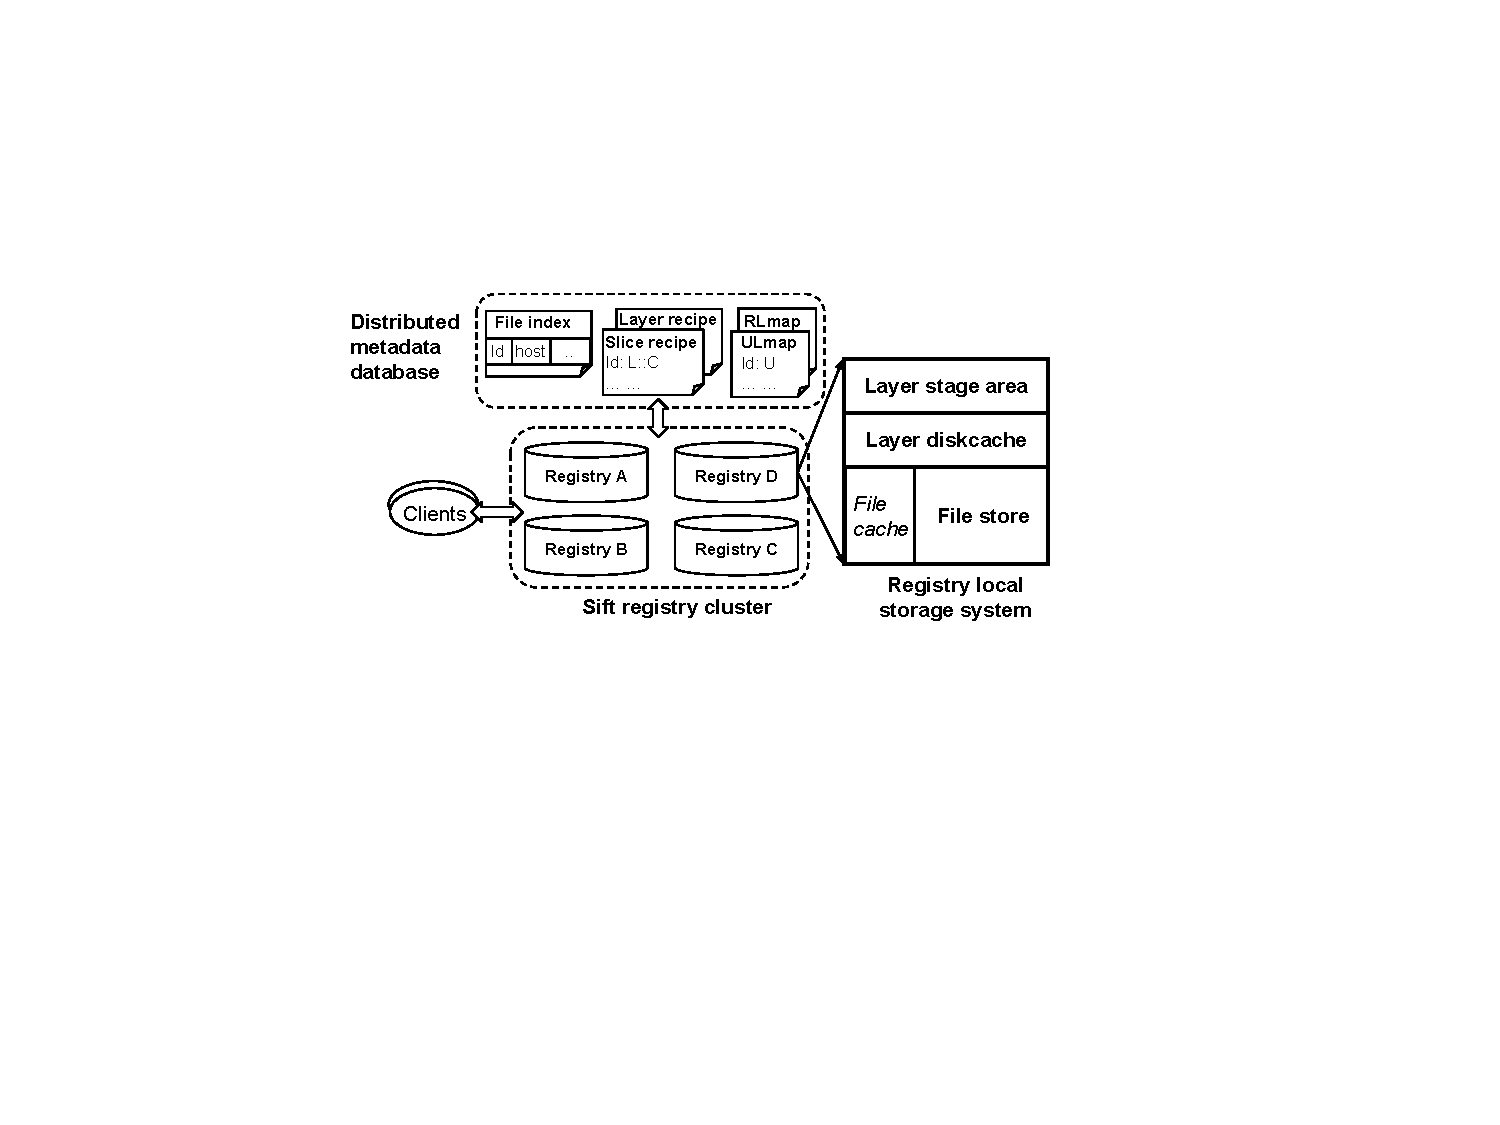
\includegraphics[width=0.9\textwidth]{graphs/sys-architecture.pdf}
%\vspace{-4pt}
			\caption{Architecture of \sysname.}
			%\label{fig:ref_count}
		%\end{minipage}
%	\begin{minipage}{0.225\textwidth}
%		\centering
%		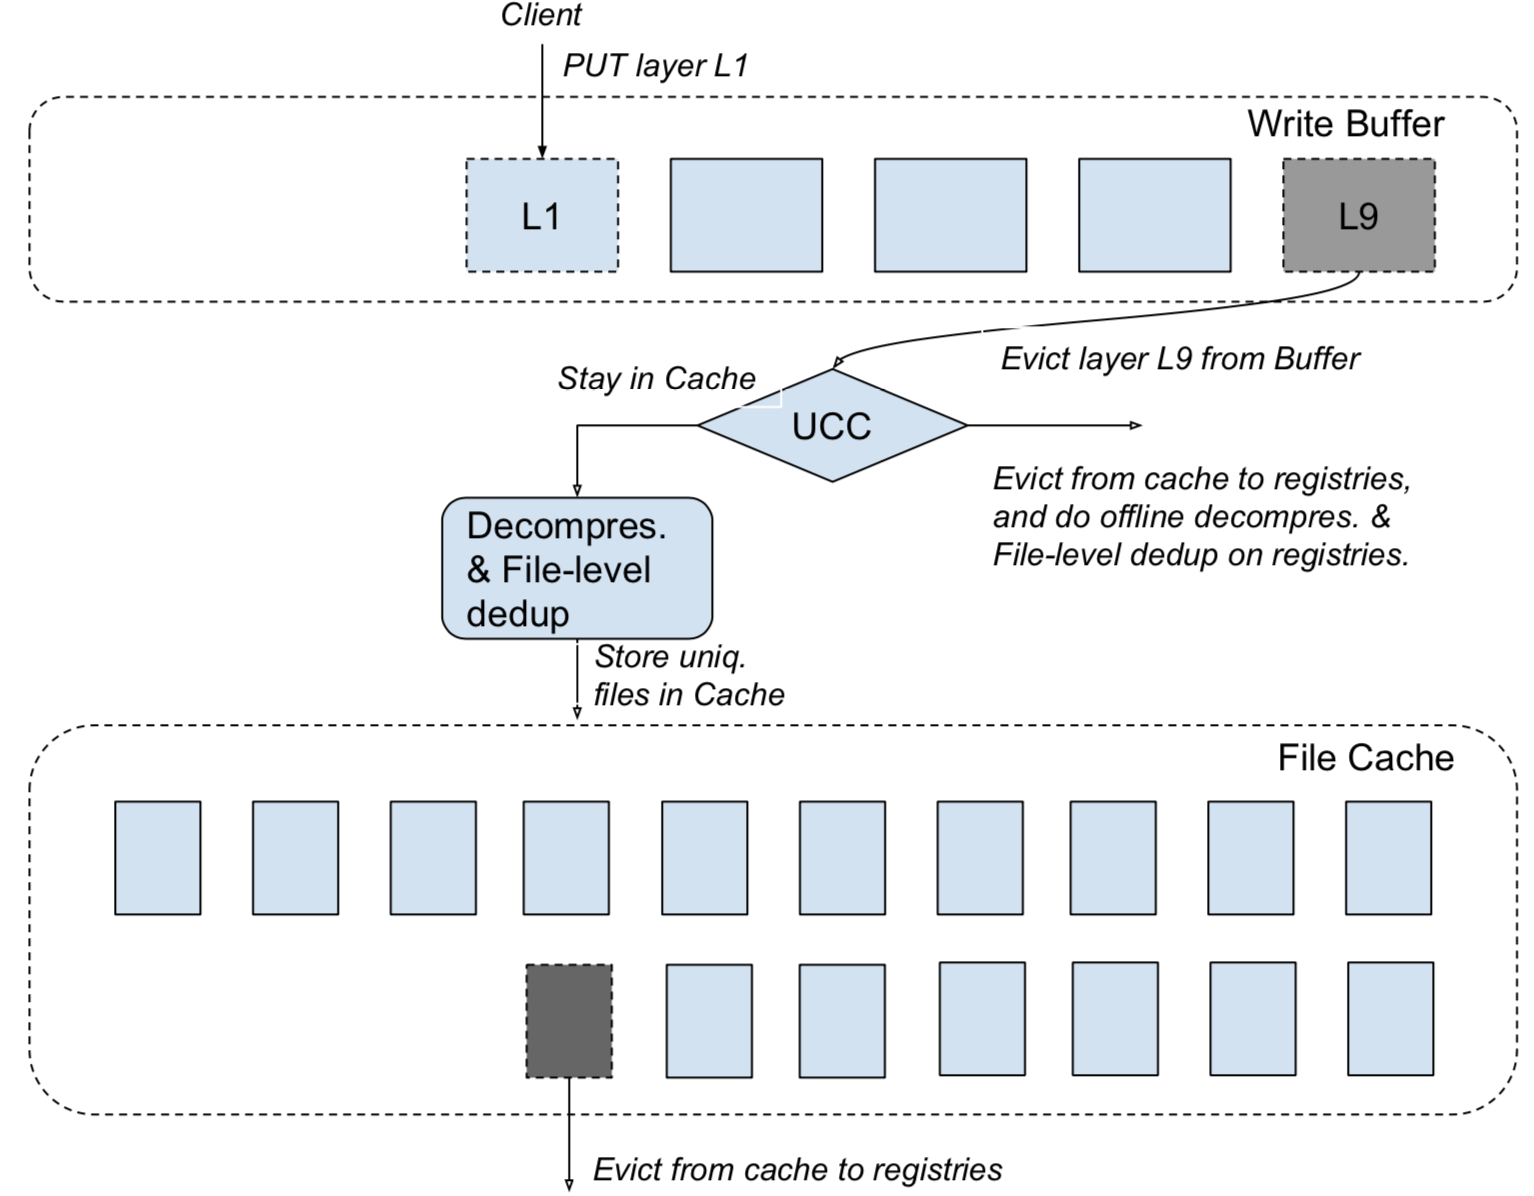
\includegraphics[width=1\textwidth]{graphs/slimmer-cache.png}
%		\caption{CDF of compress. and uncompress. layer size.}
%		\vspace{-3pt}
		\label{fig:sys-overview}
%\vspace{-4pt}
%	\end{minipage}
\end{figure*}

%We designed \sysname\ so that the interface between the Docker clients and the
%registry remains unchanged.
%
%As such, no modifications to the Docker clients are needed.
%
%Below we describe how \sysname\ handles layer pushes and
%pulls at the registry side.
%
%For the sake of this paper, we explain only the main steps omitting smaller
%details.

\sysname~seamlessly integrates the management of cache, deduplication on backend storage, and Docker registries,
and redesign the key workflows required for each functionality. 
Traditionally, caches are placed as close to the client as possible, known as proxy caches, or web/HTTP cache for temporary storing 
frequently used data to reduce server lag. 
They are typically implemented in an regional ISP or within a corporate network.
Deduplication methods are implemented on remote backend storage servers, and
transparently remove the duplicates from the incoming data stream and restore the data for read requests. 
Docker registry is a web server that serves docker pull and docker push requests.
Although docker registry is a layer-level content addressable storage system holding all the images,
it delegates storage to drivers which interact with either local file system or remote cloud storage like S3, Microsoft Azure, OpenStack Swift, and Aliyun OSS.
Intuitively, registries can be used as a proxy cache hold frequently requested layers to speedup performance 
while backend cloud storage can use deduplication to save space.
However, there are serveral unique problems about intergration of caching and deduplication to the unique workload: layers.

First, for caching layers, pull layer requests are difficult to predict because of layer reuse time is 
very long. We observed that on average around half of layers' reuse time is longer than 4 hours which means 
that if we keep a layer in cache, we might need to wait hours to get a hit.
This is because when user pulls from registry, it only pull the layers that are not stored locally. 
And consider that users might deploy their applications on different machines, so it's not easy to predict 
when the user will access which layers.
Ali Awar et.al proposed a prefetching method~\cite{anwarfast}: if there is a put layer request and subsequent get manifest request, later there will be a 
get layer request.
However, based on our trace analysis, only half of pull layer requests have a precedent put layer request within the trace collecting period, which means that
after user pushes a layer to the repository, it takes few days or weeks even months for the user to make a pull requests.
Second, for deduplicating compressed layers, the layers should first be decompressed then deduplicated while for restoring a layer, the layer's
containing files should be fetched from multiple servers and compressed together, which cause a considerable overhead for pull layer requests.

To address these issues, we propose a new user behavior based layer buffer and 
file cache to cache layers along with the unique files after decompression and deduplication.
This design considers user behaviors, such as if the users will be active later, when deciding which layer needs to be evicted from cache.
Based on our observation, user behaviours are easier to predict as shown in Figure~\ref{reusetime}.
The layer buffer stores all the newly pushed layers in memory. 
Although memory access is much faster, the size of memory is limited and considering that layer size is around few megabyte on average.
A small main memory cache cannot accommodate many active users' layers.
Hence, we couple main memory cache and flash cache to provide separate caching for layers and unique files.
When a user is inactive, we first evict its layers from layer buffer to file cache: we decompress the compressed layer, and compare its containing files
with the files that are already stored in file cache, remove the duplicate files, then store the unique files on flash storage.
In this case, flash cache can accommodate more layers than naively storing layers.
When use requests layer from file cache, the request will be separately forwarded all the servers that store its containing files, and 
compress individually and send partially layers back to user. Here, we change the Docker client interface so that when Docker client receives all partial compressed layers,
it can decompress them. Sending partially layers in parallel eliminates the network latency caused by fetching files from different servers and making a whole compressed layer.
Moreover, compressing partially layers in parallel largely mitigates compression latency caused by compressing a whole big layer since the compressing time depends on the size of uncompressed files.

    





 
